\documentclass[12pt, a4paper]{article}

% ── Packages ──────────────────────────────────────────────────────
\usepackage[utf8]{inputenc}
\usepackage[T1]{fontenc}
\usepackage{lmodern}
\usepackage[margin=1in]{geometry}
\usepackage{graphicx}
\usepackage{booktabs}
\usepackage{hyperref}
\usepackage{xcolor}
\usepackage{amsmath}
\usepackage{caption}
\usepackage{subcaption}
\usepackage{float}
\usepackage{enumitem}
\usepackage{parskip}
\usepackage{fancyhdr}
\usepackage{titlesec}
\usepackage{multirow}

\hypersetup{
  colorlinks=true,
  linkcolor=blue!60!black,
  citecolor=blue!60!black,
  urlcolor=blue!60!black,
}

% ── Headers ───────────────────────────────────────────────────────
\pagestyle{fancy}
\fancyhf{}
\fancyhead[L]{\small Pearls AQI Predictor}
\fancyhead[R]{\small \thepage}
\renewcommand{\headrulewidth}{0.4pt}

% ── Title ─────────────────────────────────────────────────────────
\title{
  \textbf{Pearls AQI Predictor} \\[0.3em]
  \large Serverless Multi-Horizon Air Quality Forecasting for Karachi \\[0.5em]
  \normalsize End-to-End ML Pipeline Report
}
\author{Abdul}
\date{September 2026}

% ══════════════════════════════════════════════════════════════════
\begin{document}
\maketitle
\thispagestyle{empty}

\begin{abstract}
This report documents the design, implementation, and evaluation of Pearls AQI Predictor --- a serverless machine learning system that forecasts the US Air Quality Index (AQI) for Karachi up to 72 hours ahead.  The system ingests hourly weather and pollutant data from the Open-Meteo API, engineers leakage-free features, trains direct per-horizon models (XGBoost, Random Forest, LSTM), and serves real-time predictions through a FastAPI backend and React dashboard.  Automation is handled by GitHub Actions (hourly feature updates, daily retraining) and deployment is managed through FastAPI Cloud and Vercel.  The best model (XGBoost) achieves an RMSE of 0.92 at the +1h horizon ($R^2 = 0.995$) and 9.41 at +24h ($R^2 = 0.511$).  Comprehensive SHAP analysis across all six forecast horizons (+1h to +72h), supported by automated staleness detection, reveals an atmospheric phase transition from short-term autoregressive persistence to synoptic meteorological forcing, while confirming the complete absence of target leakage.
\end{abstract}

\tableofcontents
\newpage

% ══════════════════════════════════════════════════════════════════
\section{Introduction}

Air pollution is a serious public health concern in Karachi, Pakistan's largest city.  The US Air Quality Index (AQI) condenses concentrations of multiple pollutants into a single number that communicates health risk to the public.  This project builds a complete, serverless pipeline that:

\begin{enumerate}
  \item Collects hourly weather and pollutant data from a free public API.
  \item Engineers time-aware features and stores them in a cloud feature store.
  \item Trains separate ML models for six forecast horizons (1h, 6h, 12h, 24h, 48h, 72h).
  \item Serves forecasts through a REST API and an interactive web dashboard.
  \item Automates the entire cycle with GitHub Actions.
\end{enumerate}

The goal is to predict the AQI for the \emph{next three days} with enough accuracy to be useful for health advisories, while keeping the infrastructure entirely serverless and free-tier friendly.


% ══════════════════════════════════════════════════════════════════
\section{Data Sources and Collection}

\subsection{Open-Meteo API}

All data comes from the \textbf{Open-Meteo API} (\texttt{open-meteo.com}), which provides free, keyless access to both weather and air quality observations and numerical forecasts.  Open-Meteo was chosen because it provides weather and air quality from a single source, includes a 3-day meteorological forecast API (essential for direct multi-day prediction), and has generous rate limits suitable for automated pipelines.

Two types of hourly variables are fetched:

\begin{itemize}
  \item \textbf{Weather variables} (6): temperature (2m), relative humidity (2m), precipitation, sea-level pressure, wind speed (10m), and wind direction (10m).
  \item \textbf{Air quality variables} (7): PM\textsubscript{2.5}, PM\textsubscript{10}, CO, NO\textsubscript{2}, SO\textsubscript{2}, O\textsubscript{3}, and the US AQI (the prediction target).
\end{itemize}

\subsection{Location}

The system is configured for \textbf{Karachi} (24.86\textdegree N, 67.01\textdegree E), an arid coastal megacity with severe particulate burdens (mean AQI $\approx 88$).  The geographical coordinates are configurable through environment variables to facilitate multi-city expansion.

\subsection{Historical Backfill}

A one-time backfill pipeline (\texttt{backfill.py}) populated the feature store with three years of historical hourly observations (September 2023 -- September 2026, totaling 26,496 rows).  To respect API chunking constraints, historical data was processed in 90-day segments with a 4-day rolling overlap buffer, ensuring that lag and rolling statistics (up to 72 hours) compute continuously across boundaries.


% ══════════════════════════════════════════════════════════════════
\section{Exploratory Data Analysis}

Exploratory Data Analysis (EDA) was performed across two phases: an initial distribution and correlation screening (\texttt{01\_eda\_open\_meteo\_aqi.ipynb}) and advanced time-series decomposition and autocorrelation modeling (\texttt{eda\_advanced.py}).

\subsection{Target Variable Distribution and Outliers}

The US AQI for Karachi exhibits the summary statistics in Table~\ref{tab:eda_stats}.

\begin{table}[H]
\centering
\caption{US AQI descriptive statistics (3-year dataset, 26,496 hourly rows).}
\label{tab:eda_stats}
\begin{tabular}{lr}
\toprule
\textbf{Statistic} & \textbf{Value} \\
\midrule
Mean   & 88.0 \\
Std    & 22.0 \\
Min    & 41 \\
Median & 82 \\
Max    & 173 \\
\bottomrule
\end{tabular}
\end{table}

The distribution is moderately right-skewed, with the majority of values falling in the EPA ``Moderate'' category (51--100) and an extended tail reaching into ``Unhealthy'' (151--200).  Figure~\ref{fig:eda_outliers} illustrates the empirical distribution, seasonal boxplots, and outlier boundaries.

\begin{figure}[H]
\centering
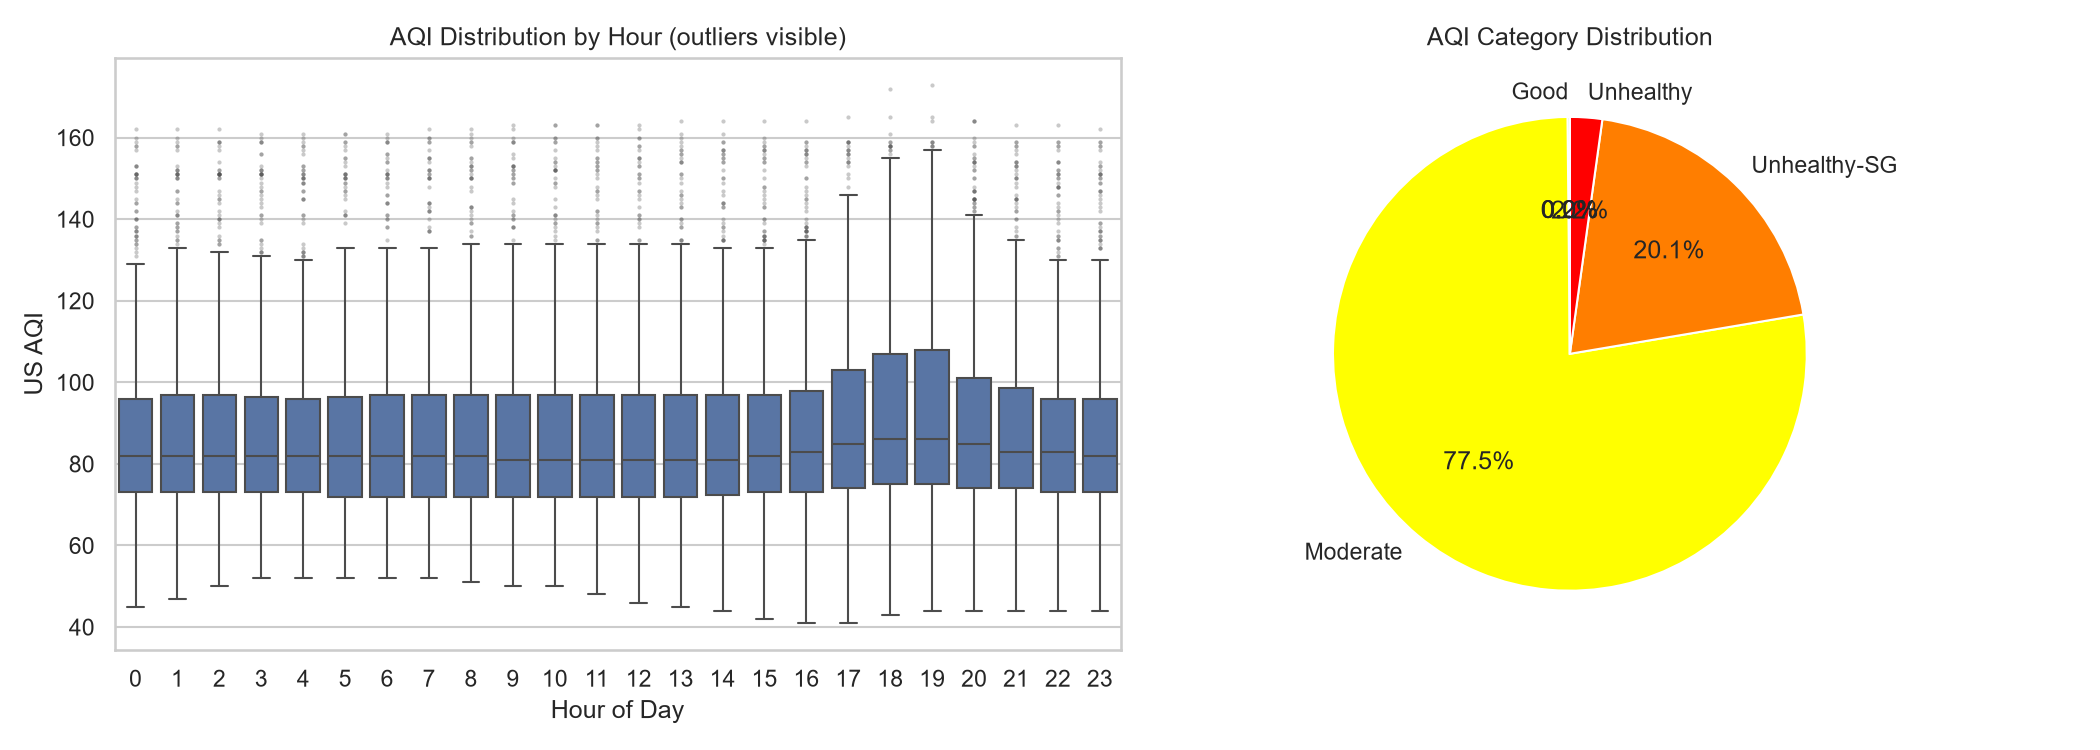
\includegraphics[width=0.88\linewidth]{eda_outliers.png}
\caption{Distribution and outlier analysis for Karachi AQI, showing right-skewed density and seasonal concentration percentiles.}
\label{fig:eda_outliers}
\end{figure}

\subsection{Temporal Dynamics: Diurnal and Seasonal Cycles}

Time-series decomposition reveals two dominant periodicities:
\begin{itemize}
  \item \textbf{Diurnal Cycle}: As shown in Figure~\ref{fig:eda_daily}, AQI peaks reliably between 7:00 PM and 10:00 PM ($\sim$96 AQI).  This occurs when evening commute emissions coincide with the collapse of the planetary boundary layer at sunset, trapping vehicular and industrial exhaust near ground level.  AQI reaches its minimum in the early morning before sunrise.
  \item \textbf{Seasonal Cycle}: AQI is substantially higher and more volatile during winter (November--February) due to persistent thermal inversions and calm continental winds.  Conversely, during the summer monsoon (July--September), marine boundary layer ventilation and precipitation scavenging wash out suspended particulates.
\end{itemize}

\begin{figure}[H]
\centering
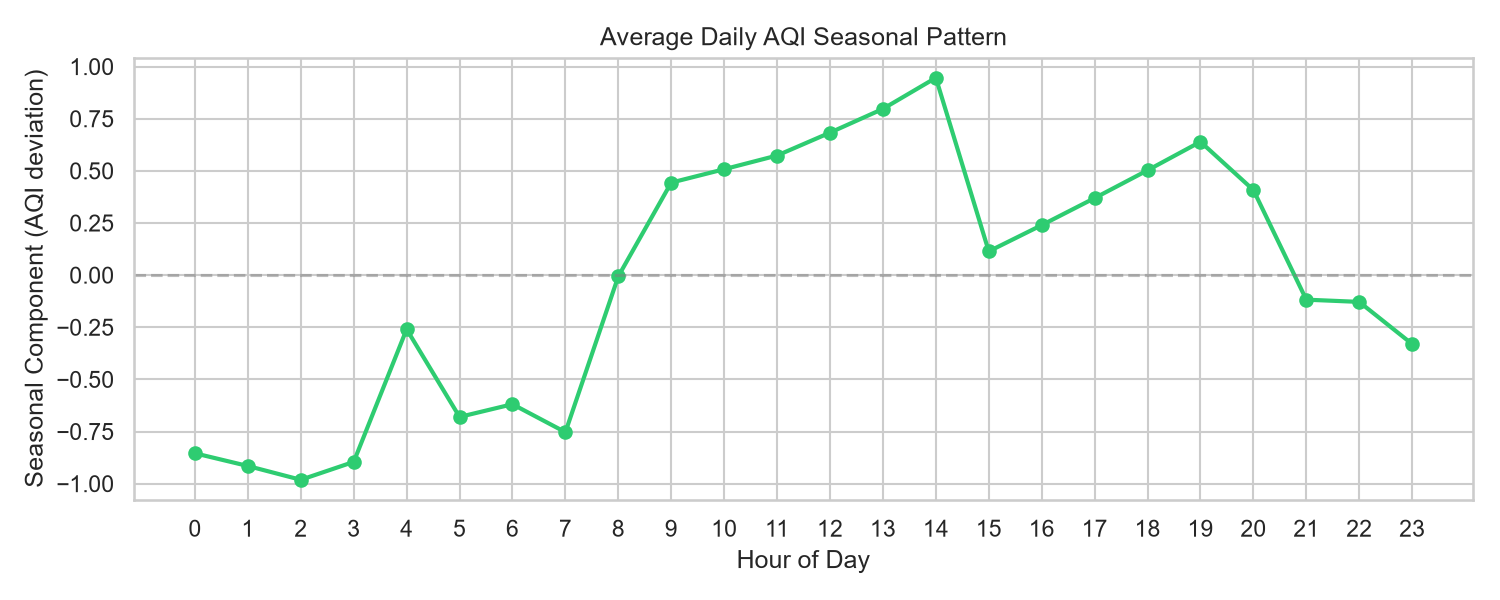
\includegraphics[width=0.88\linewidth]{eda_daily_pattern.png}
\caption{Diurnal hourly AQI profile for Karachi, highlighting morning and evening rush-hour concentration spikes.}
\label{fig:eda_daily}
\end{figure}

Figure~\ref{fig:eda_stl} displays the Seasonal-Trend decomposition using LOESS (STL).  The decomposition confirms that seasonal oscillations account for substantial variance, while multi-week trend movements reflect regional air mass shifts.

\begin{figure}[H]
\centering
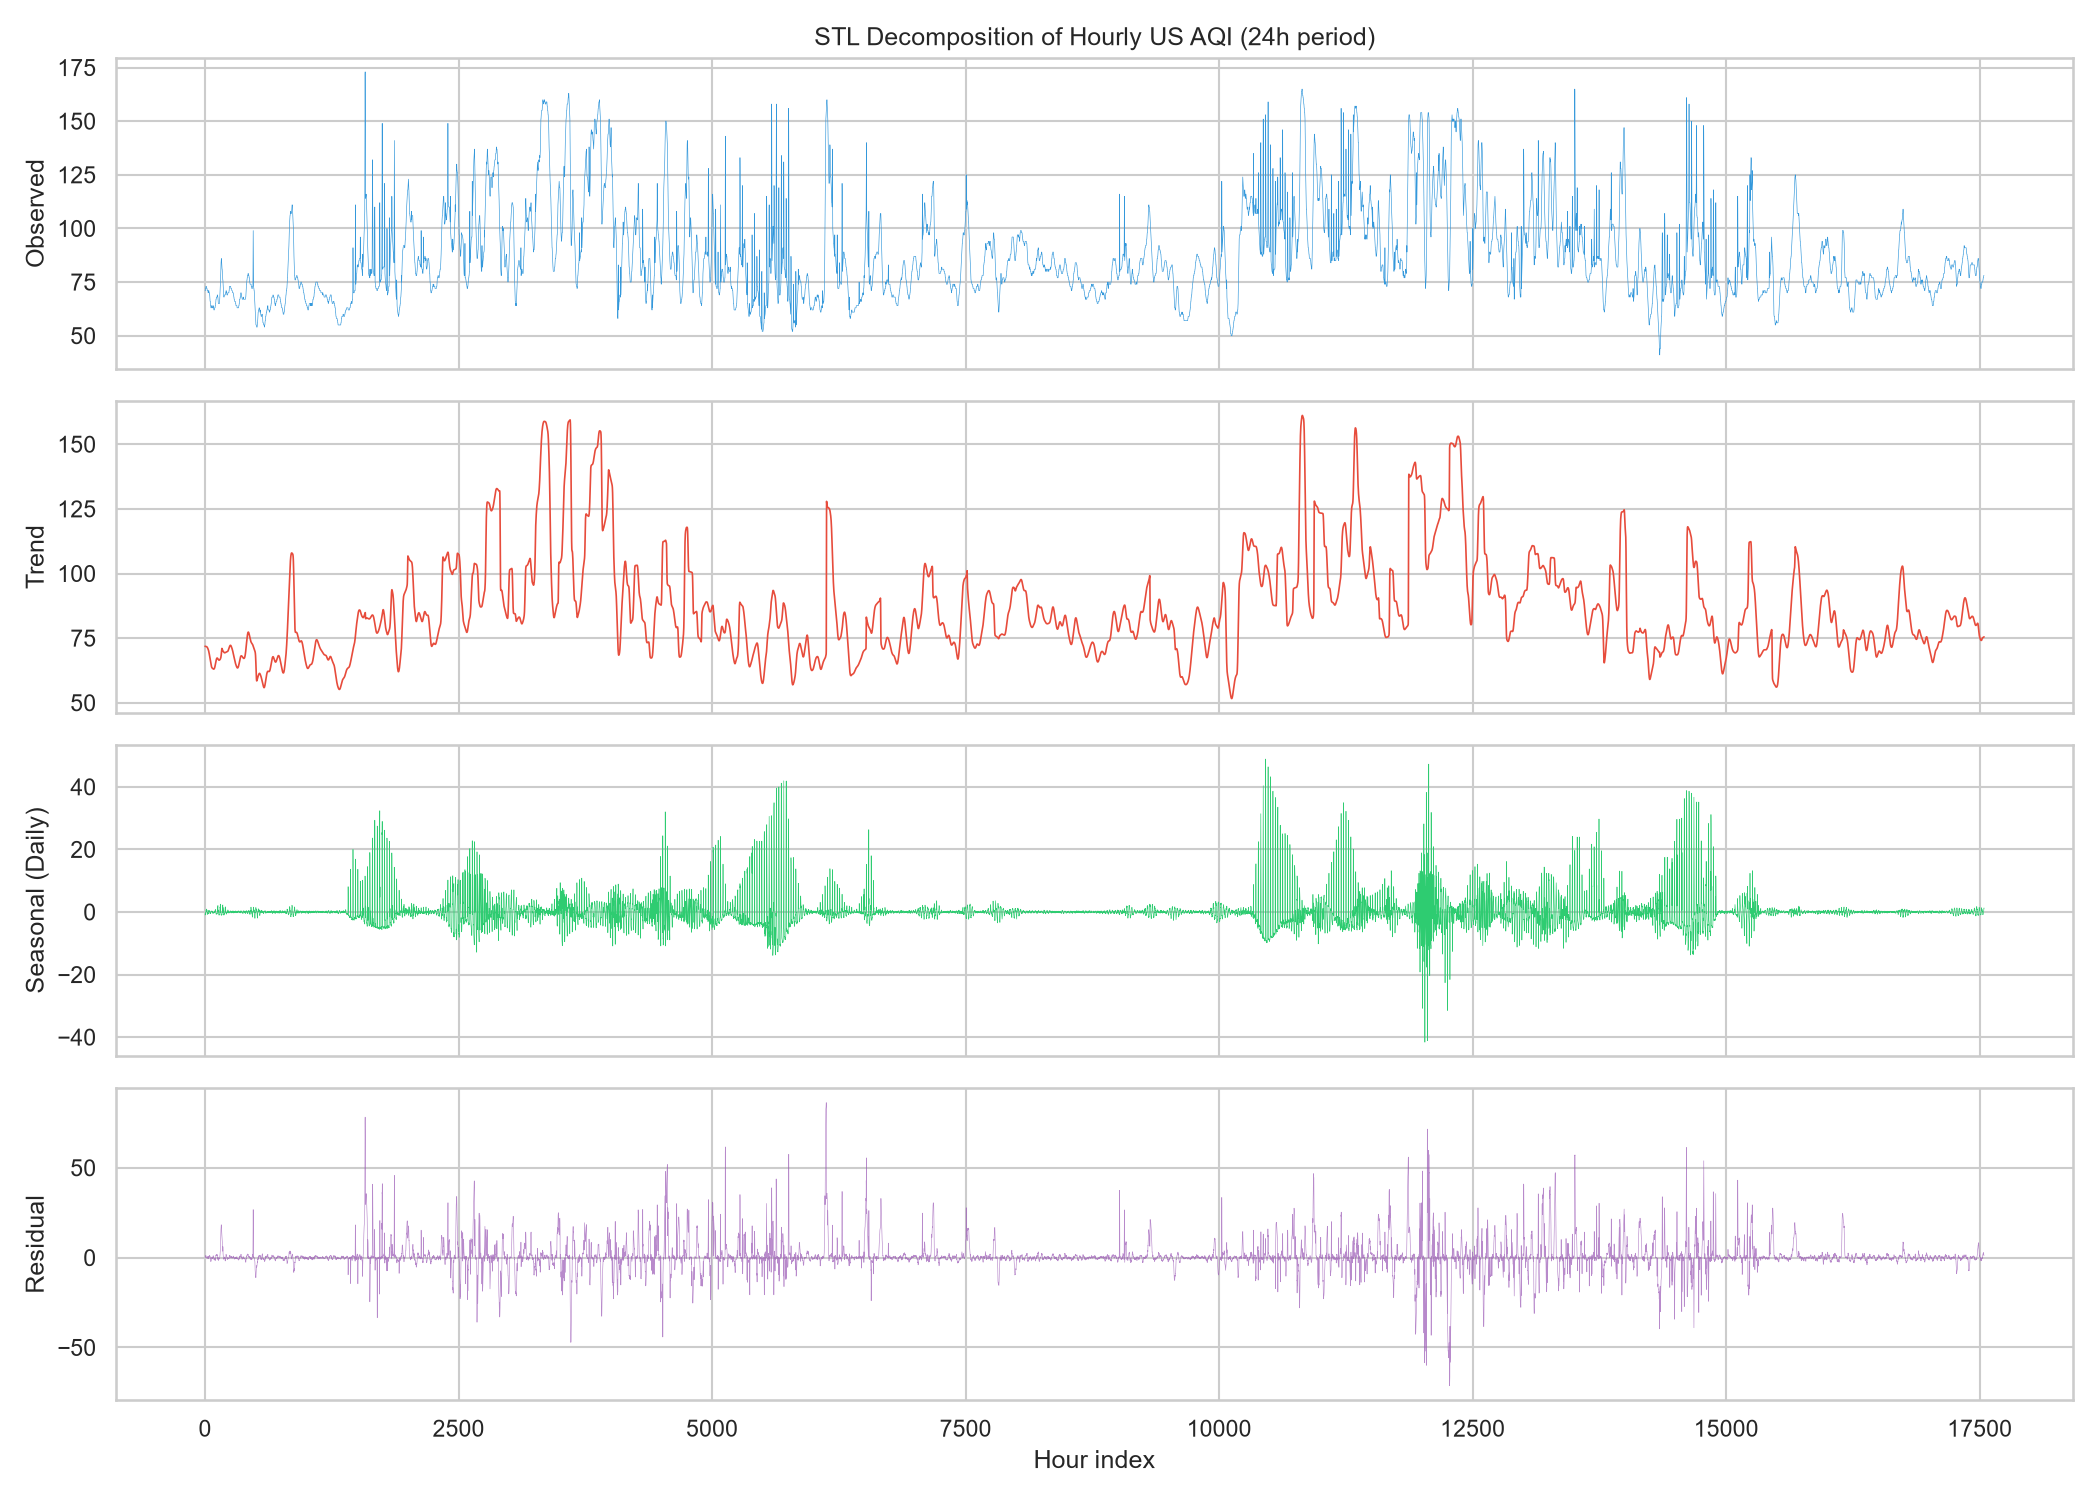
\includegraphics[width=0.92\linewidth]{eda_stl_decomposition.png}
\caption{Seasonal-Trend Decomposition using LOESS (STL) of hourly AQI, isolating trend, seasonal cyclicity, and stochastic residuals.}
\label{fig:eda_stl}
\end{figure}

\subsection{Stationarity and Autocorrelation Structure}

The Augmented Dickey-Fuller (ADF) test rejected the unit root null hypothesis ($p \ll 0.001$), confirming stationarity.  Figure~\ref{fig:eda_acf_pacf} shows the Autocorrelation Function (ACF) and Partial Autocorrelation Function (PACF) up to 72 lags.  The ACF demonstrates strong persistence, remaining at 0.440 even at lag 72.  The PACF displays pronounced spikes at 24h, 48h, and 72h, demonstrating sharp diurnal resonance.  This empirical evidence justifies the explicit incorporation of 24h, 48h, and 72h lag and rolling features.

\begin{figure}[H]
\centering
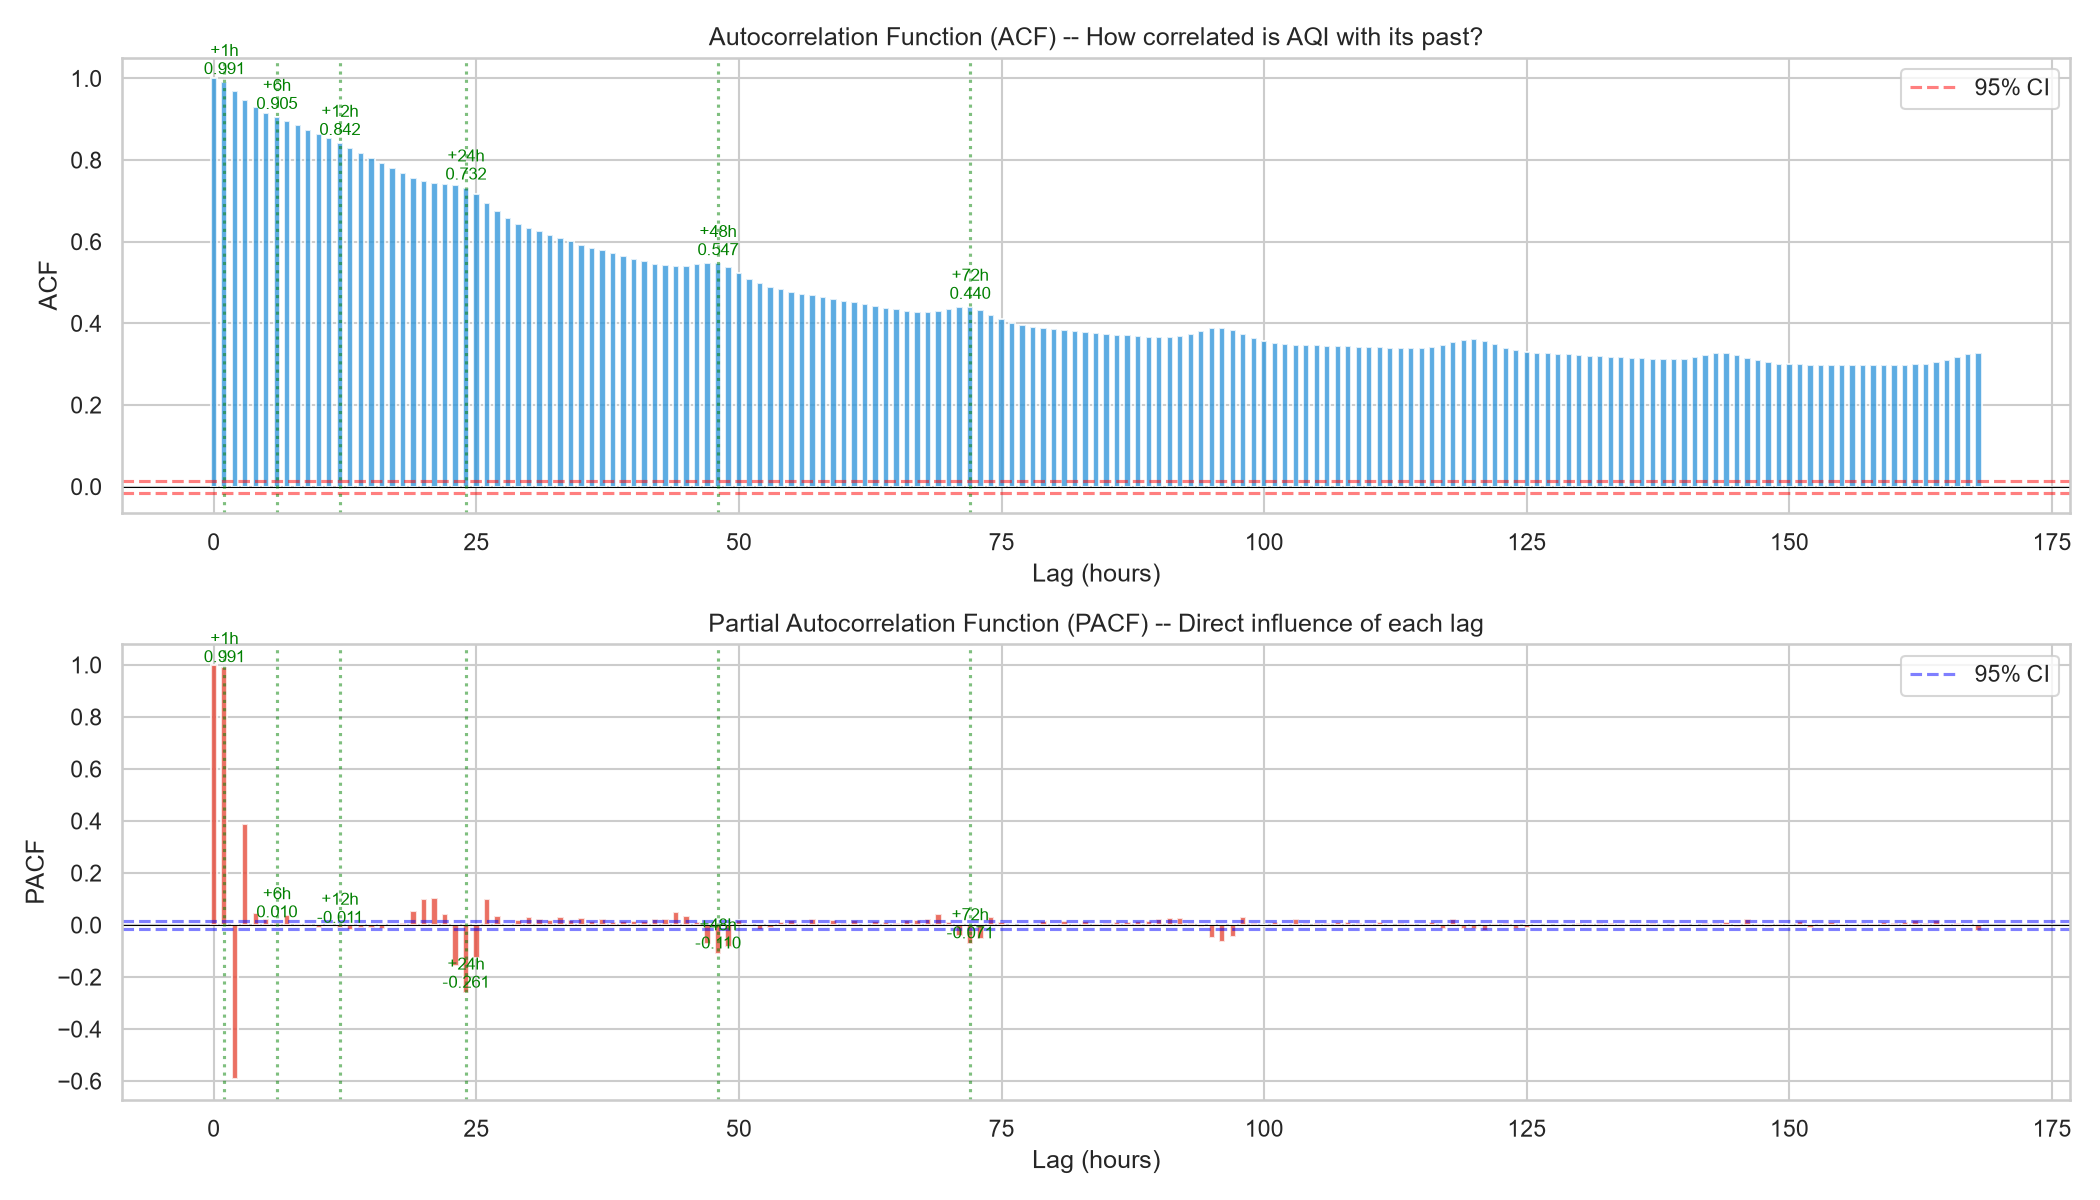
\includegraphics[width=0.9\linewidth]{eda_acf_pacf.png}
\caption{ACF and PACF of Karachi hourly AQI across 72 lags, exhibiting persistence and diurnal spikes at multiples of 24 hours.}
\label{fig:eda_acf_pacf}
\end{figure}


% ══════════════════════════════════════════════════════════════════
\section{Feature Engineering}
\label{sec:features}

Feature engineering is performed by \texttt{build\_features.py}, converting 13 raw variables into 60+ leakage-free predictive signals structured into six functional categories:

\subsection{Cyclical Temporal Encodings}
Hours (0--23), months (1--12), and days of the week (0--6) are encoded via trigonometric pairs:
\begin{equation}
  x_{\sin} = \sin\left(\frac{2\pi \cdot t}{T}\right), \quad x_{\cos} = \cos\left(\frac{2\pi \cdot t}{T}\right)
\end{equation}
This ensures that boundary transitions (e.g., hour 23 to 0, or December to January) maintain smooth continuous distance.  A binary \texttt{is\_weekend} flag captures economic activity shifts.

\subsection{Target Autoregressive Lags}
Lagged target features are generated at $t - 1$, $t - 3$, $t - 6$, $t - 12$, $t - 24$, $t - 48$, and $t - 72$ hours.  The extended 48h and 72h lags capture multi-day diurnal persistence identified in the PACF analysis.

\subsection{Rolling and Statistical Aggregations}
Rolling means (3h, 6h, 12h, 24h, 48h), rolling standard deviation (6h, 24h), rolling extrema (24h min/max), and exponentially weighted moving averages (EWMA with 12h half-life) summarize volatility and air mass trajectory.  Critically, all rolling windows are \textbf{shifted by 1 hour} ($t - 1$) to prevent target leakage.

\subsection{Pollutant Lags and Leakage Prevention}
The US AQI is a deterministic piecewise linear function of instantaneous pollutant concentrations ($PM_{2.5}, PM_{10}, O_3, NO_2, SO_2, CO$).  Consequently, feeding current-timestep pollutant concentrations into the feature matrix constitutes severe target leakage.  In this pipeline, \textbf{all current raw pollutant concentrations are dropped}.  Only historical lags ($t-1, t-24$) and rolling aggregates (6h, 12h, 24h) are preserved as valid state features.

\subsection{Trend and Momentum Indicators}
First differences ($\Delta \text{AQI}_{1\text{h}}, \Delta \text{AQI}_{3\text{h}}, \Delta \text{AQI}_{6\text{h}}, \Delta \text{AQI}_{24\text{h}}$) and deviations from rolling baselines capture atmospheric acceleration and dispersion momentum.

\subsection{Atmospheric Physics and Weather Interactions}
\begin{itemize}
  \item \textbf{Wind Vector Decomposition}: Wind speed ($s$) and meteorological direction ($\theta$) are converted into orthogonal Cartesian vectors ($u = -s \sin \theta, v = -s \cos \theta$) to enable linear boundary layer modeling.
  \item \textbf{Particulate Formation Proxy}: The temperature-humidity interaction index ($T \times RH / 100$) models secondary inorganic aerosol nucleation under humid coastal conditions.
  \item \textbf{Precipitation Indicators}: Cumulative rainfall over 6 hours and binary 24-hour wash-out indicators account for wet deposition scavenging.
\end{itemize}


% ══════════════════════════════════════════════════════════════════
\section{Feature Store Architecture}

Features are registered in \textbf{Hopsworks Feature Store} (\texttt{aqi\_features}, version 2).  The feature group uses \texttt{time} as both primary key and event-time stamp, stored in Apache Hudi format to support ACID upserts, time-travel queries, and reproducible dataset snapshotting.  An insert-with-retry handler manages transient HTTP connectivity in cloud automation.


% ══════════════════════════════════════════════════════════════════
\section{Direct Multi-Horizon Modeling}
\label{sec:modeling}

\subsection{Direct vs.\ Recursive Formulation}

Instead of a recursive single-step autoregressive model that feeds noisy predictions back into itself across 72 iterations, the system deploys a \textbf{direct multi-horizon forecasting architecture}.  Six autonomous models are trained for discrete horizons:
\begin{equation}
  \hat{y}_{t+h} = f_h(\mathbf{x}_t, \mathbf{w}_{t+h}), \quad h \in \{1, 6, 12, 24, 48, 72\}
\end{equation}
Intermediate hourly forecasts (e.g., +2h through +5h) are linearly interpolated between bounding direct models.

\subsection{Numerical Forecast Weather and Delta Features}

At time $t$, Open-Meteo provides 3-day weather forecasts.  These future meteorological signals are integrated into the horizon models by shifting weather features by $-h$ steps ($\mathbf{w}_{t+h}$).  Furthermore, meteorological deltas ($\Delta \mathbf{w}_h = \mathbf{w}_{t+h} - \mathbf{w}_t$) supply the model with expected changes in sea breeze, humidity, and barometric pressure over the forecast window.

\subsection{Horizon-Specific Feature Pruning}

For immediate horizons ($h \le 6$), short-term lags ($t-1$, $t-3$) are highly predictive.  For extended horizons ($h \ge 24$), high-frequency lags decay into stochastic noise.  To prevent overfitting, features are pruned per horizon: the 24h, 48h, and 72h models discard 1h/3h lags and focus on 24h diurnal cycles, rolling baselines, and forecast weather deltas.

\subsection{Model Candidates and Validation Split}

Three model families were benchmarked across all horizons:
\begin{enumerate}
  \item \textbf{XGBoost}: 500 gradient-boosted trees, max depth 6, learning rate 0.05, early stopping on validation loss.
  \item \textbf{Random Forest}: 300 bagged trees, max depth 15, square-root feature subsampling.
  \item \textbf{PyTorch LSTM}: 2-layer recurrent network (128 hidden units), 48-hour sliding window, Huber loss ($\delta=10$), Adam optimizer.
\end{enumerate}
Data is split chronologically: 70\% train (18,547 rows), 15\% validation (3,974 rows), 15\% test (3,975 rows), preserving temporal causality.


% ══════════════════════════════════════════════════════════════════
\section{Benchmark Results and Analysis}

\subsection{Evaluation Metrics}

Table~\ref{tab:results} summarizes the test-set performance across all models and horizons.  XGBoost achieved the highest accuracy across every horizon.

\begin{table}[H]
\centering
\caption{Test-set performance comparison. Bold highlights winning models.}
\label{tab:results}
\small
\begin{tabular}{llrrr}
\toprule
\textbf{Horizon} & \textbf{Model} & \textbf{RMSE} & \textbf{MAE} & \textbf{$R^2$} \\
\midrule
\multirow{3}{*}{+1h}
  & \textbf{XGBoost}     & \textbf{0.92} & \textbf{0.46} & \textbf{0.995} \\
  & Random Forest        & 1.12          & 0.48          & 0.993 \\
  & LSTM                 & 1.73          & 0.82          & 0.984 \\
\midrule
\multirow{3}{*}{+6h}
  & \textbf{XGBoost}     & \textbf{3.94} & \textbf{2.03} & \textbf{0.914} \\
  & Random Forest        & 4.74          & 2.28          & 0.876 \\
  & LSTM                 & 4.89          & 2.50          & 0.869 \\
\midrule
\multirow{3}{*}{+12h}
  & \textbf{XGBoost}     & \textbf{6.34} & \textbf{3.57} & \textbf{0.778} \\
  & Random Forest        & 6.76          & 3.78          & 0.748 \\
  & LSTM                 & 7.05          & 4.09          & 0.728 \\
\midrule
\multirow{3}{*}{+24h}
  & \textbf{XGBoost}     & \textbf{9.41} & \textbf{6.25} & \textbf{0.511} \\
  & Random Forest        & 9.61          & 6.38          & 0.490 \\
  & LSTM                 & 9.82          & 6.69          & 0.472 \\
\midrule
\multirow{3}{*}{+48h}
  & \textbf{XGBoost}     & \textbf{12.07} & \textbf{8.29} & \textbf{0.200} \\
  & Random Forest        & 12.28          & 8.49          & 0.172 \\
  & LSTM                 & 14.26          & 9.83          & $-$0.136 \\
\midrule
\multirow{3}{*}{+72h}
  & \textbf{XGBoost}     & \textbf{12.60} & \textbf{8.90} & \textbf{0.131} \\
  & Random Forest        & 13.25          & 9.25          & 0.040 \\
  & LSTM                 & 13.00          & 9.09          & 0.042 \\
\bottomrule
\end{tabular}
\end{table}

\subsection{Performance Degradation Analysis}

Predictive error scales with horizon distance:
\begin{itemize}
  \item At +1h, error is negligible (RMSE 0.92, $R^2 = 0.995$), capturing atmospheric inertia.
  \item At +6h and +12h, strong fidelity is retained ($R^2 = 0.914$ and $0.778$), aiding same-day public alerts.
  \item At +24h, the model maintains operational utility ($R^2 = 0.511$, RMSE 9.41), accurately tracking diurnal peak-trough shifts.
  \item Beyond 24h, predictability decays ($R^2 = 0.200$ at +48h, $0.131$ at +72h).  Multi-day air quality is inherently governed by unpredictable local emissions (e.g., traffic fluctuations, unannounced industrial activity) and mesoscale weather forecast drift.  The leveling off from +48h to +72h (RMSE 12.07 to 12.60) indicates the models converge gracefully toward the seasonal climatological mean.
  \item XGBoost outperforms naive baselines (persistence, climatological mean, same-hour-yesterday) across all horizons.
\end{itemize}


% ══════════════════════════════════════════════════════════════════
\section{Explainability with Multi-Horizon SHAP}
\label{sec:shap}

\subsection{Automated Staleness Detection and Refresh Pipeline}

The pipeline implements an automated staleness detection architecture (\texttt{is\_horizon\_stale}).  Before running TreeExplainer, the system inspects each horizon's serialized output reports against the modification timestamp of the corresponding model artifact (\texttt{model.pkl}).  If a model has been retrained or an output artifact is missing, SHAP recalculation is triggered automatically.  If up-to-date, redundant computations are bypassed, ensuring efficiency during CI/CD runs.

\subsection{Cross-Horizon Feature Dynamics}

Figure~\ref{fig:shap_evolution} charts the cross-horizon evolution of feature importance from +1h to +72h.  A clear physical phase transition is observed: autoregressive lags dominate immediate predictions, while future weather forecasts and seasonal cyclical components take over at longer lead times.

\begin{figure}[H]
\centering
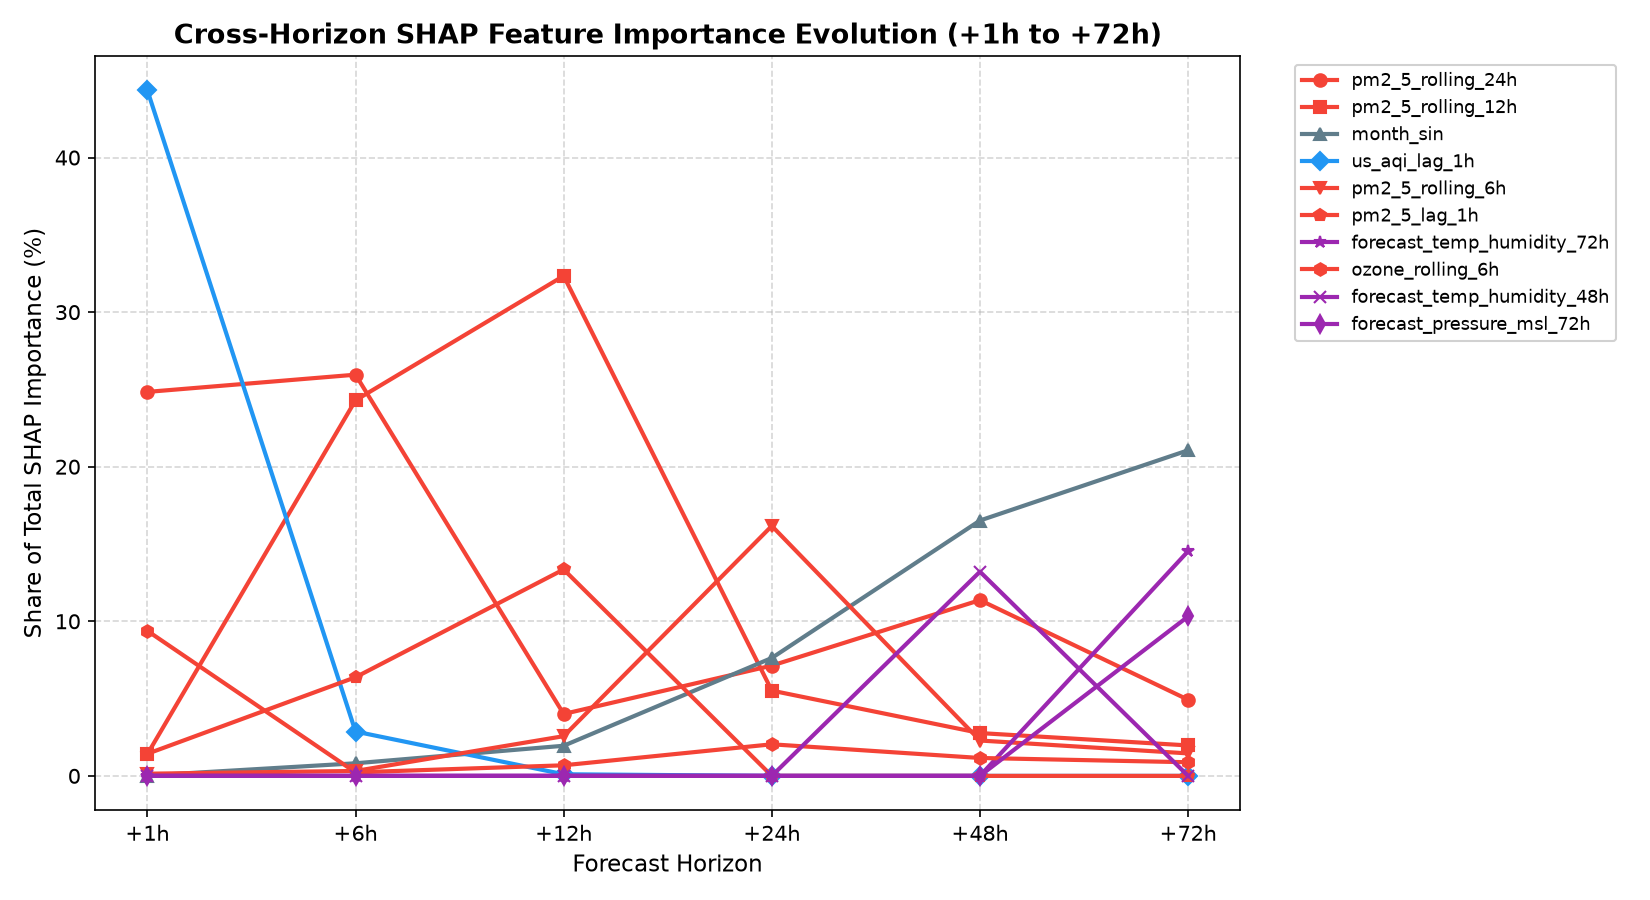
\includegraphics[width=0.95\linewidth]{shap_cross_horizon_evolution.png}
\caption{Cross-horizon SHAP feature importance evolution (+1h to +72h). Autoregressive lags dictate short-term predictions, transitioning to numerical weather forecasts and seasonal dynamics at multi-day horizons.}
\label{fig:shap_evolution}
\end{figure}

Table~\ref{tab:shap_categories} quantifies the distribution of mean absolute SHAP importance across functional categories.

\begin{table}[H]
\centering
\caption{Category share of total SHAP importance (\%) across forecast horizons.}
\label{tab:shap_categories}
\small
\begin{tabular}{lrrrrrr}
\toprule
\textbf{Feature Category} & \textbf{+1h} & \textbf{+6h} & \textbf{+12h} & \textbf{+24h} & \textbf{+48h} & \textbf{+72h} \\
\midrule
AQI Lags                  & 37.8\% & 11.2\% &  4.7\% &  4.5\% &  2.5\% &  2.0\% \\
Pollutant Lags/Rolling    & 46.3\% & 62.4\% & 62.4\% & 44.7\% & 26.6\% & 15.0\% \\
AQI Rolling Statistics    &  6.9\% &  6.2\% &  3.5\% &  5.9\% &  3.6\% &  3.5\% \\
Trend / Momentum          &  3.8\% &  4.8\% &  2.8\% &  7.8\% &  5.2\% &  4.4\% \\
Current Weather           &  0.4\% &  1.5\% &  4.9\% &  6.1\% &  5.0\% &  4.8\% \\
Forecast Weather / Deltas &  0.0\% &  4.6\% & 10.8\% & 21.0\% & 36.2\% & 44.1\% \\
Cyclical Time Features    &  4.8\% &  9.3\% & 11.0\% & 10.1\% & 20.8\% & 26.2\% \\
\bottomrule
\end{tabular}
\end{table}

\subsection{Horizon Feature Rankings}

Tables~\ref{tab:shap_1h}, \ref{tab:shap_24h}, and \ref{tab:shap_72h} list the dominant features for the immediate (+1h), diurnal (+24h), and extended (+72h) models.

\begin{table}[H]
\centering
\caption{Top features for the +1h XGBoost model by mean absolute SHAP value.}
\label{tab:shap_1h}
\small
\begin{tabular}{lr}
\toprule
\textbf{Feature} & \textbf{Mean $|$SHAP$|$} \\
\midrule
\texttt{us\_aqi\_lag\_1h}       & 9.854 \\
\texttt{pm2\_5\_rolling\_24h}   & 5.519 \\
\texttt{ozone\_rolling\_6h}     & 2.085 \\
\texttt{aqi\_rolling\_3h}       & 1.183 \\
\texttt{aqi\_change\_1h}        & 1.044 \\
\texttt{pm2\_5\_lag\_1h}         & 0.317 \\
\texttt{pm2\_5\_rolling\_12h}   & 0.313 \\
\texttt{pm2\_5\_lag\_24h}        & 0.221 \\
\bottomrule
\end{tabular}
\end{table}

\begin{table}[H]
\centering
\caption{Top features for the +24h XGBoost model by mean absolute SHAP value.}
\label{tab:shap_24h}
\small
\begin{tabular}{lr}
\toprule
\textbf{Feature} & \textbf{Mean $|$SHAP$|$} \\
\midrule
\texttt{pm2\_5\_rolling\_6h}           & 5.261 \\
\texttt{month\_sin}                    & 2.482 \\
\texttt{pm2\_5\_rolling\_24h}          & 2.321 \\
\texttt{forecast\_temp\_humidity\_24h} & 1.996 \\
\texttt{pm2\_5\_rolling\_12h}          & 1.795 \\
\texttt{aqi\_change\_6h}               & 1.481 \\
\texttt{pm10\_rolling\_6h}             & 1.027 \\
\texttt{nitrogen\_dioxide\_rolling\_6h} & 0.975 \\
\texttt{aqi\_trend\_24h}               & 0.854 \\
\texttt{forecast\_wind\_speed\_10m\_24h} & 0.809 \\
\texttt{forecast\_wind\_u\_24h}        & 0.775 \\
\bottomrule
\end{tabular}
\end{table}

\begin{table}[H]
\centering
\caption{Top features for the +72h XGBoost model by mean absolute SHAP value.}
\label{tab:shap_72h}
\small
\begin{tabular}{lr}
\toprule
\textbf{Feature} & \textbf{Mean $|$SHAP$|$} \\
\midrule
\texttt{month\_sin}                    & 4.616 \\
\texttt{forecast\_temp\_humidity\_72h} & 3.186 \\
\texttt{forecast\_pressure\_msl\_72h}  & 2.260 \\
\texttt{forecast\_wind\_u\_72h}        & 1.361 \\
\texttt{pm2\_5\_rolling\_24h}          & 1.080 \\
\texttt{delta\_temp\_humidity\_72h}    & 1.053 \\
\texttt{pressure\_msl}                 & 0.652 \\
\texttt{hour\_cos}                     & 0.607 \\
\texttt{aqi\_change\_6h}               & 0.501 \\
\texttt{pm2\_5\_rolling\_12h}          & 0.432 \\
\bottomrule
\end{tabular}
\end{table}

Figure~\ref{fig:shap_horizons} contrasts feature importance bar plots across the +1h, +24h, and +72h horizons, highlighting the progression from immediate air mass persistence to synoptic meteorological forcing.

\begin{figure}[H]
\centering
\begin{subfigure}[b]{0.32\linewidth}
  \centering
  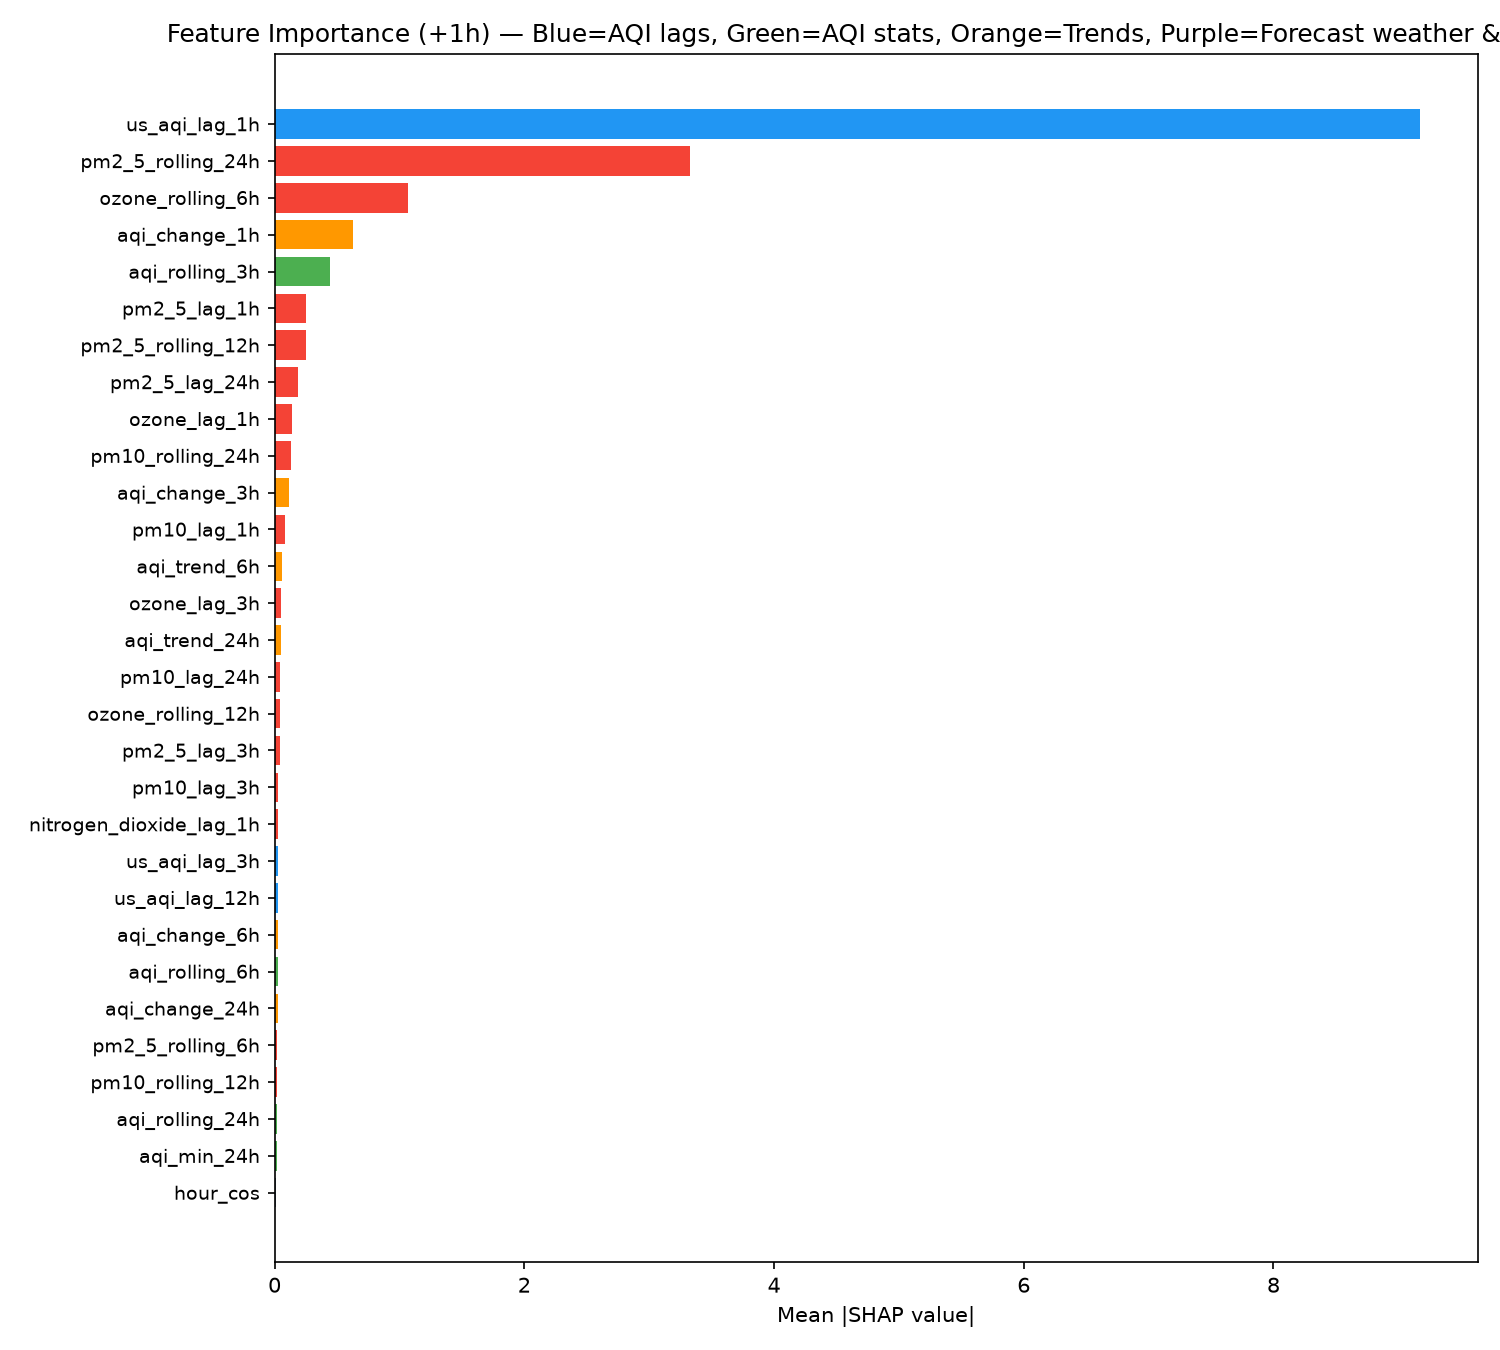
\includegraphics[width=\linewidth]{shap_importance_1h.png}
  \caption{+1h Immediate Horizon}
  \label{fig:shap_bar_1h}
\end{subfigure}
\hfill
\begin{subfigure}[b]{0.32\linewidth}
  \centering
  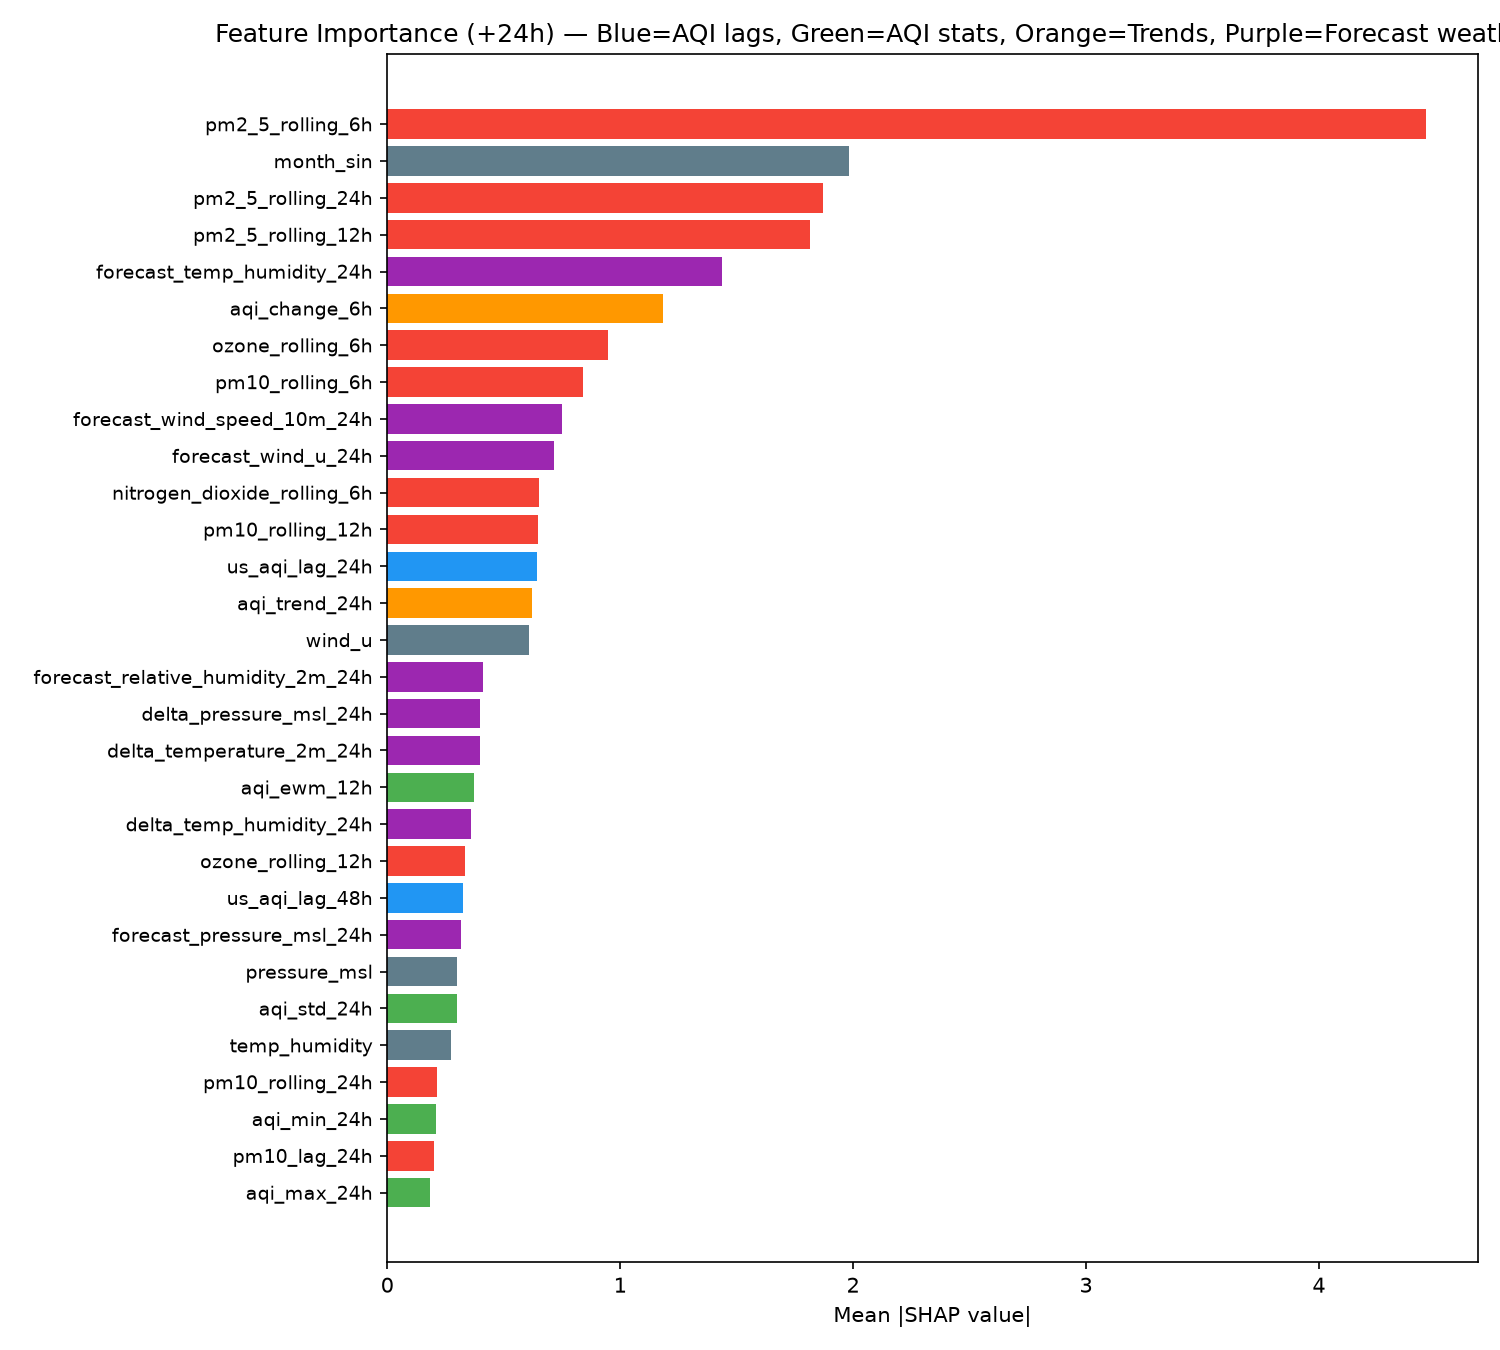
\includegraphics[width=\linewidth]{shap_importance_24h.png}
  \caption{+24h Diurnal Horizon}
  \label{fig:shap_bar_24h}
\end{subfigure}
\hfill
\begin{subfigure}[b]{0.32\linewidth}
  \centering
  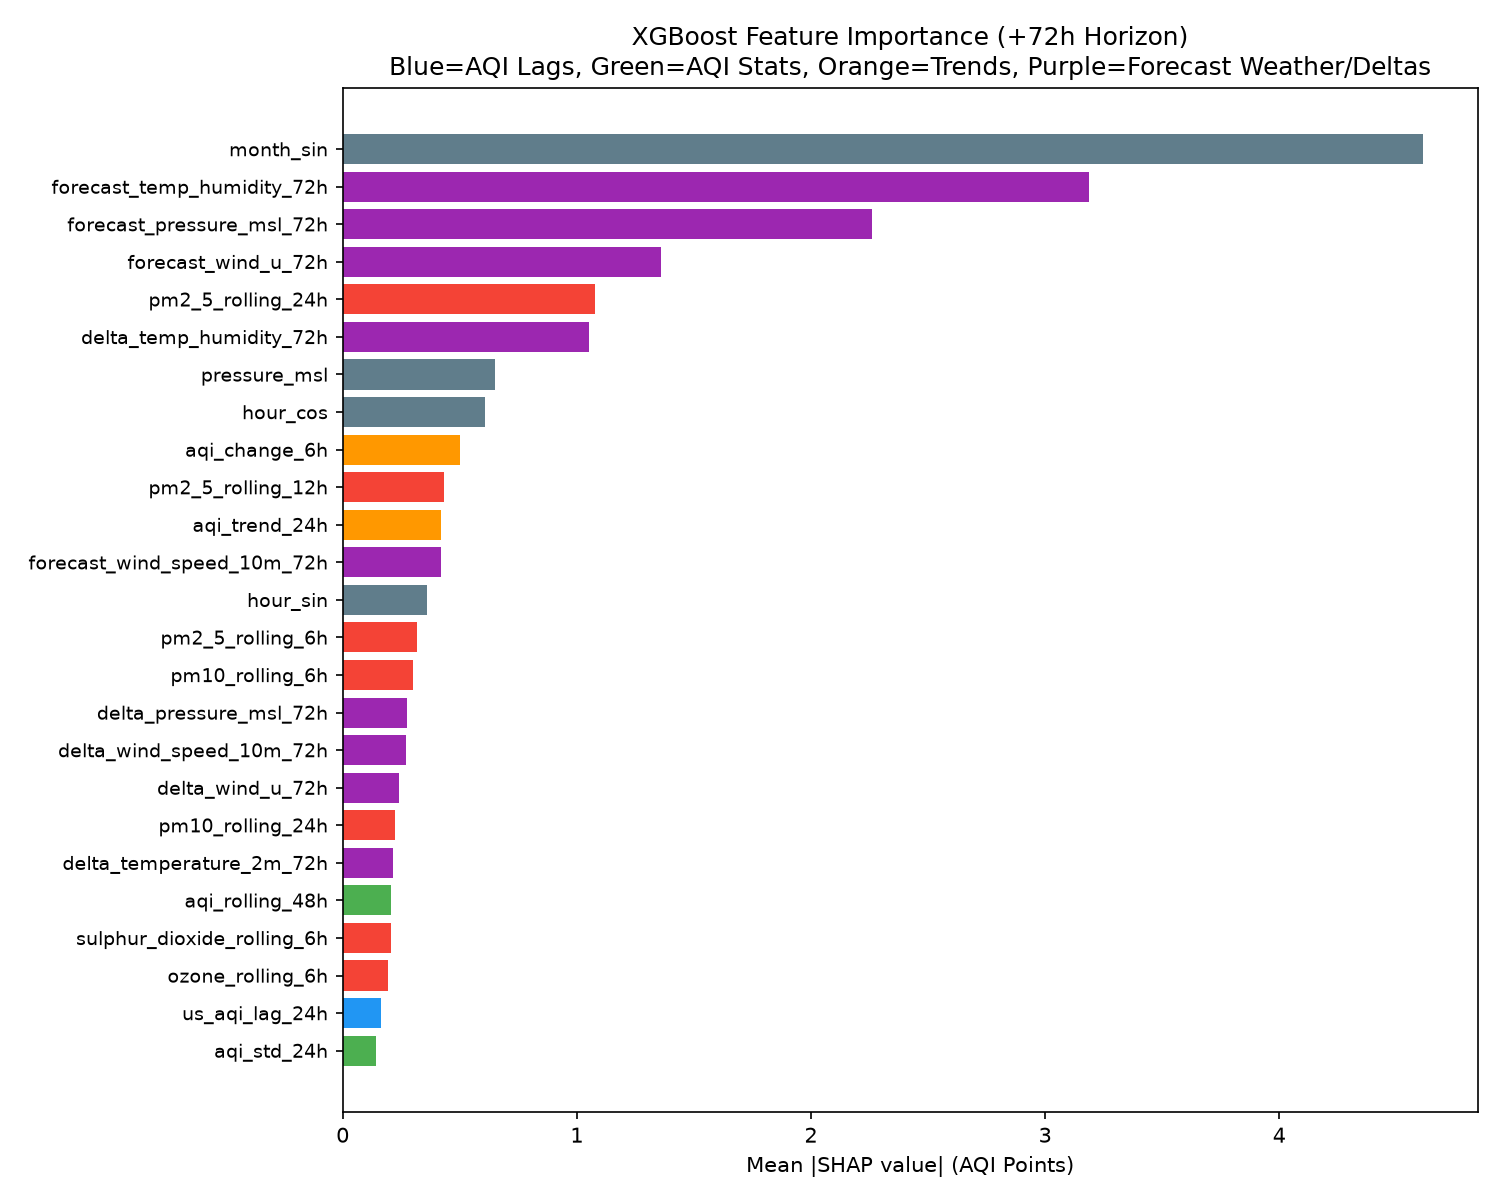
\includegraphics[width=\linewidth]{shap_importance_72h.png}
  \caption{+72h 3-Day Horizon}
  \label{fig:shap_bar_72h}
\end{subfigure}
\caption{SHAP feature importance bar charts across forecast horizons, color-coded by category: blue (AQI lags), green (rolling aggregates), orange (trends), purple (forecast weather and deltas).}
\label{fig:shap_horizons}
\end{figure}

\subsection{Summary Distribution and Directionality}

Figure~\ref{fig:shap_summary_24h} displays the beeswarm summary plot for the +24h diurnal model.  High values of \texttt{forecast\_temp\_humidity\_24h} push AQI higher (secondary aerosol formation), whereas elevated sea-breeze wind vectors (\texttt{forecast\_wind\_u\_24h}) exert a negative SHAP impact (coastal dispersion).  Positive \texttt{month\_sin} values drive higher winter baseline predictions.

\begin{figure}[H]
\centering
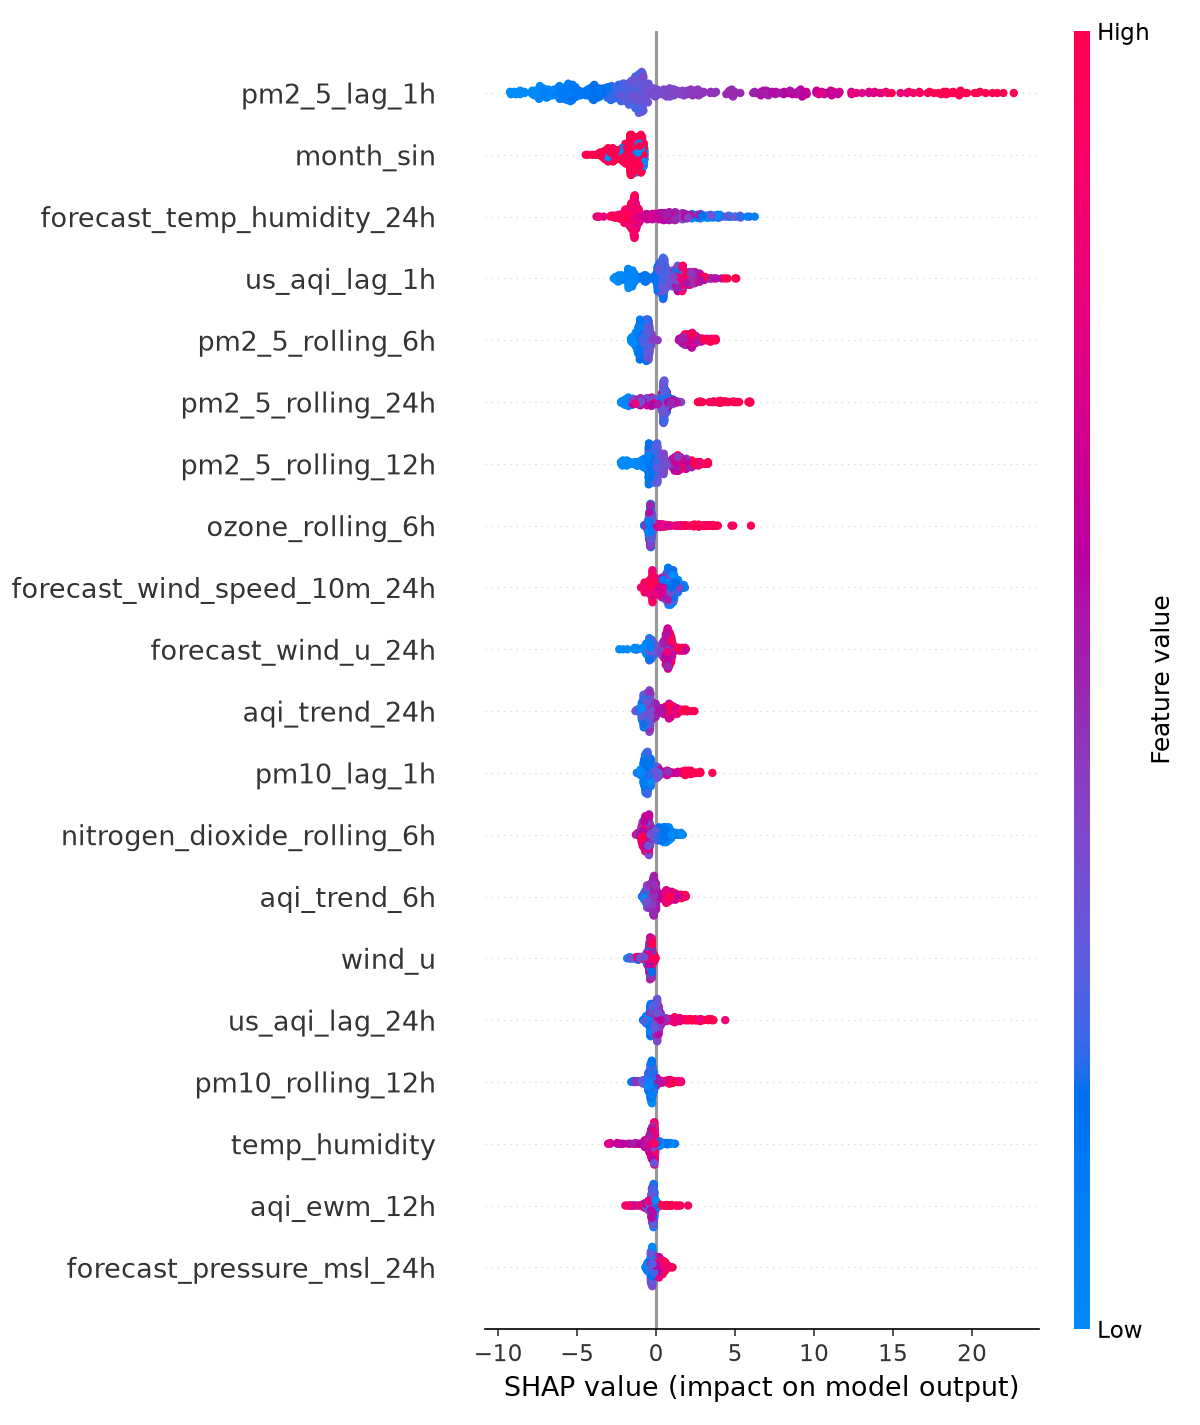
\includegraphics[width=0.88\linewidth]{shap_summary_24h.png}
\caption{SHAP beeswarm summary plot for the +24h diurnal model, showing feature value distributions and positive/negative impact directions.}
\label{fig:shap_summary_24h}
\end{figure}

\textbf{Target Leakage Verification}: Across all 6 models, zero raw pollutant features (\texttt{pm2\_5}, \texttt{pm10}, \texttt{ozone}) appear in the top rankings, confirming that the pipeline is strictly leakage-free.


% ══════════════════════════════════════════════════════════════════
\section{System Architecture and Deployment}

The production system is organized into four decoupled layers:

\subsection{Data and Ingestion Layer}
\texttt{sources.py} queries the Open-Meteo archive and forecast endpoints, aligning meteorological and air quality records on standardized UTC hourly timestamps.

\subsection{Feature Store Layer}
\texttt{hopsworks\_utils.py} connects to Hopsworks via environment credentials, handles feature group schemas, and inserts updates with exponential backoff.

\subsection{Inference and Serving Layer (Backend)}
A \textbf{FastAPI} application (\texttt{api.py}) serves inference:
\begin{itemize}
  \item \texttt{/api/current}: Real-time AQI with EPA category, severity rating, and dominant pollutant.
  \item \texttt{/api/forecast}: Direct multi-horizon forecasts up to +72h with hourly linear interpolation.
  \item \texttt{/api/history}: 48-hour trailing observed measurements for context.
  \item \texttt{/api/analytics}: Dynamic telemetry returning model benchmark metrics and SHAP importance for all 6 horizons.
\end{itemize}
The backend is hosted on \textbf{FastAPI Cloud} with automatic continuous deployment on repository commits, accompanied by an in-memory 5-minute TTL cache to minimize external API overhead.

\subsection{User Interface (Dashboard)}
The dashboard is built with \textbf{React}, \textbf{TypeScript}, \textbf{Vite}, and \textbf{Tailwind CSS v4}, visualizing forecasts via \textbf{Recharts}.  It includes an interactive multi-horizon explainability panel allowing users to inspect SHAP drivers across any horizon (+1h through +72h).  The frontend is hosted on \textbf{Vercel} with proxy rewrites to the FastAPI Cloud backend.


% ══════════════════════════════════════════════════════════════════
\section{Continuous Integration and Pipeline Automation}

Automation is managed through \textbf{GitHub Actions} (\texttt{.github/workflows/pipelines.yml}):
\begin{itemize}
  \item \textbf{Hourly Feature Pipeline}: Runs every hour at minute 0 (cron \texttt{0\ *\ *\ *\ *}), ingesting recent actuals and forecasts, computing engineered features, and upserting them to Hopsworks. Dependencies are isolated in \texttt{requirements-feature.txt} (excluding heavy ML libraries) to finish in under 2 minutes.
  \item \textbf{Daily Training Pipeline}: Runs daily at 02:00 UTC (cron \texttt{0\ 2\ *\ *\ *}) following the feature update, retraining direct XGBoost and Random Forest models, updating metrics, and committing fresh artifacts to Git.
  \item \textbf{Continuous Deployment}: Model artifact commits trigger automated backend image rebuilds on FastAPI Cloud, providing an autonomous retrain-and-deploy loop.
\end{itemize}


% ══════════════════════════════════════════════════════════════════
\section{Architectural Trade-offs and Engineering Insights}

\begin{enumerate}[label=\textbf{\arabic*.}]
  \item \textbf{Direct Multi-Horizon vs.\ Autoregressive Chaining}: While recursive models require only a single training run, early prediction errors compound exponentially across 72 steps.  The direct approach requires managing six distinct models, but eliminates error propagation and enables horizon-specific feature pruning.

  \item \textbf{Gradient Boosted Trees vs.\ Deep Sequence Models}: XGBoost demonstrated superior sample efficiency and accuracy over PyTorch LSTM across all horizons, achieving lower RMSE at a fraction of the computational footprint ($\sim$2 seconds vs.\ $\sim$45 minutes training time).  Tree-based architectures are well suited for tabular atmospheric features, whereas LSTMs require extensive sequence normalization and struggle with long-range multi-day tabular dependencies.

  \item \textbf{Leakage Prevention vs.\ Feature Richness}: Eliminating instantaneous pollutant concentrations prevents trivial target leakage.  Retaining lagged derivatives and rolling windows enables the model to capture air mass history while enforcing strict physical causality.

  \item \textbf{Serverless Cloud vs.\ Persistent Infrastructure}: Integrating Open-Meteo, Hopsworks, GitHub Actions, FastAPI Cloud, and Vercel delivers production-grade ML capability with zero fixed server hosting fees and minimal maintenance overhead.
\end{enumerate}


% ══════════════════════════════════════════════════════════════════
\section{Limitations and Future Work}

\subsection{Current Limitations}
\begin{itemize}
  \item \textbf{Multi-Day Forecast Ceiling}: Beyond 24 hours, $R^2$ decreases to $0.13$--$0.20$.  Predicting mesoscale air quality 3 days ahead remains fundamentally bounded by localized emission uncertainties.
  \item \textbf{Single-Location Scope}: The current deployment is optimized for Karachi.  Multi-city scaling requires spatial embeddings or regionalized feature groups.
  \item \textbf{Static Hyperparameters}: Model hyperparameters were tuned via validation search but remain fixed.  Automated hyperparameter optimization (e.g., Optuna) in CI would enhance adaptability.
\end{itemize}

\subsection{Future Enhancements}
\begin{itemize}
  \item Integration of satellite aerosol optical depth (AOD) observations from Copernicus/CAMS.
  \item Conformal prediction intervals to output calibrated uncertainty bounds alongside point forecasts.
  \item Automated push alert webhooks triggered when forecasted AQI crosses hazardous EPA thresholds.
\end{itemize}


% ══════════════════════════════════════════════════════════════════
\section{Technology Stack Summary}

Table~\ref{tab:tech_stack} lists the technology stack used across all project layers.

\begin{table}[H]
\centering
\caption{System technology stack summary.}
\label{tab:tech_stack}
\begin{tabular}{ll}
\toprule
\textbf{Subsystem} & \textbf{Technologies} \\
\midrule
Language             & Python 3.12 \\
Machine Learning     & XGBoost, scikit-learn, PyTorch \\
Feature Store        & Hopsworks (Apache Hudi) \\
Model Registry       & Hopsworks Model Registry \\
Data Source          & Open-Meteo Weather \& Air Quality APIs \\
Backend Framework    & FastAPI, Uvicorn, Pydantic v2 \\
Frontend Stack       & React, TypeScript, Vite, Tailwind CSS v4, Recharts \\
Workflow CI/CD       & GitHub Actions \\
Cloud Hosting        & FastAPI Cloud (Backend), Vercel (Frontend) \\
Explainability / EDA & SHAP, Matplotlib, Seaborn, statsmodels \\
\bottomrule
\end{tabular}
\end{table}


% ══════════════════════════════════════════════════════════════════
\section{Conclusion}

The Pearls AQI Predictor provides a robust, leakage-free, end-to-end machine learning system for 72-hour air quality forecasting in Karachi.  By pairing direct multi-horizon gradient boosted trees with Open-Meteo numerical weather forecasts and an automated serverless workflow, the system achieves strong accuracy at near-term horizons (RMSE 0.92 at +1h, 3.94 at +6h) and actionable diurnal guidance at +24h (RMSE 9.41, $R^2 = 0.511$).  Comprehensive SHAP explainability across all six forecast horizons confirms that the models transition logically from autoregressive inertia to synoptic meteorological forcing, offering transparent and physically grounded intelligence for public health decision-making.

\end{document}
